\documentclass[twoside]{book}

% Packages required by doxygen
\usepackage{calc}
\usepackage{doxygen}
\usepackage{graphicx}
\usepackage[utf8]{inputenc}
\usepackage{makeidx}
\usepackage{multicol}
\usepackage{multirow}
\usepackage{textcomp}
\usepackage[table]{xcolor}

% Font selection
\usepackage[T1]{fontenc}
\usepackage{mathptmx}
\usepackage[scaled=.90]{helvet}
\usepackage{courier}
\usepackage{amssymb}
\usepackage{sectsty}
\renewcommand{\familydefault}{\sfdefault}
\allsectionsfont{%
  \fontseries{bc}\selectfont%
  \color{darkgray}%
}
\renewcommand{\DoxyLabelFont}{%
  \fontseries{bc}\selectfont%
  \color{darkgray}%
}

% Page & text layout
\usepackage{geometry}
\geometry{%
  a4paper,%
  top=2.5cm,%
  bottom=2.5cm,%
  left=2.5cm,%
  right=2.5cm%
}
\tolerance=750
\hfuzz=15pt
\hbadness=750
\setlength{\emergencystretch}{15pt}
\setlength{\parindent}{0cm}
\setlength{\parskip}{0.2cm}
\makeatletter
\renewcommand{\paragraph}{%
  \@startsection{paragraph}{4}{0ex}{-1.0ex}{1.0ex}{%
    \normalfont\normalsize\bfseries\SS@parafont%
  }%
}
\renewcommand{\subparagraph}{%
  \@startsection{subparagraph}{5}{0ex}{-1.0ex}{1.0ex}{%
    \normalfont\normalsize\bfseries\SS@subparafont%
  }%
}
\makeatother

% Headers & footers
\usepackage{fancyhdr}
\pagestyle{fancyplain}
\fancyhead[LE]{\fancyplain{}{\bfseries\thepage}}
\fancyhead[CE]{\fancyplain{}{}}
\fancyhead[RE]{\fancyplain{}{\bfseries\leftmark}}
\fancyhead[LO]{\fancyplain{}{\bfseries\rightmark}}
\fancyhead[CO]{\fancyplain{}{}}
\fancyhead[RO]{\fancyplain{}{\bfseries\thepage}}
\fancyfoot[LE]{\fancyplain{}{}}
\fancyfoot[CE]{\fancyplain{}{}}
\fancyfoot[RE]{\fancyplain{}{\bfseries\scriptsize Generated on Wed Jan 18 2017 16\-:10\-:31 for gnss\-\_\-odom\-\_\-new by Doxygen }}
\fancyfoot[LO]{\fancyplain{}{\bfseries\scriptsize Generated on Wed Jan 18 2017 16\-:10\-:31 for gnss\-\_\-odom\-\_\-new by Doxygen }}
\fancyfoot[CO]{\fancyplain{}{}}
\fancyfoot[RO]{\fancyplain{}{}}
\renewcommand{\footrulewidth}{0.4pt}
\renewcommand{\chaptermark}[1]{%
  \markboth{#1}{}%
}
\renewcommand{\sectionmark}[1]{%
  \markright{\thesection\ #1}%
}

% Indices & bibliography
\usepackage{natbib}
\usepackage[titles]{tocloft}
\setcounter{tocdepth}{3}
\setcounter{secnumdepth}{5}
\makeindex

% Hyperlinks (required, but should be loaded last)
\usepackage{ifpdf}
\ifpdf
  \usepackage[pdftex,pagebackref=true]{hyperref}
\else
  \usepackage[ps2pdf,pagebackref=true]{hyperref}
\fi
\hypersetup{%
  colorlinks=true,%
  linkcolor=blue,%
  citecolor=blue,%
  unicode%
}

% Custom commands
\newcommand{\clearemptydoublepage}{%
  \newpage{\pagestyle{empty}\cleardoublepage}%
}


%===== C O N T E N T S =====

\begin{document}

% Titlepage & ToC
\hypersetup{pageanchor=false}
\pagenumbering{roman}
\begin{titlepage}
\vspace*{7cm}
\begin{center}%
{\Large gnss\-\_\-odom\-\_\-new }\\
\vspace*{1cm}
{\large Generated by Doxygen 1.8.6}\\
\vspace*{0.5cm}
{\small Wed Jan 18 2017 16:10:31}\\
\end{center}
\end{titlepage}
\clearemptydoublepage
\tableofcontents
\clearemptydoublepage
\pagenumbering{arabic}
\hypersetup{pageanchor=true}

%--- Begin generated contents ---
\chapter{Class Index}
\section{Class List}
Here are the classes, structs, unions and interfaces with brief descriptions\-:\begin{DoxyCompactList}
\item\contentsline{section}{\hyperlink{struct_coord_sys}{Coord\-Sys} }{\pageref{struct_coord_sys}}{}
\item\contentsline{section}{\hyperlink{class_c_t_f}{C\-T\-F} }{\pageref{class_c_t_f}}{}
\item\contentsline{section}{\hyperlink{classfeedback}{feedback} }{\pageref{classfeedback}}{}
\item\contentsline{section}{\hyperlink{class_k_f}{K\-F} }{\pageref{class_k_f}}{}
\item\contentsline{section}{\hyperlink{structkf___ft_qt}{kf\-\_\-\-Ft\-Qt} }{\pageref{structkf___ft_qt}}{}
\item\contentsline{section}{\hyperlink{structkf___hk_rk}{kf\-\_\-\-Hk\-Rk} }{\pageref{structkf___hk_rk}}{}
\item\contentsline{section}{\hyperlink{structkf___xk_pk}{kf\-\_\-\-Xk\-Pk} }{\pageref{structkf___xk_pk}}{}
\item\contentsline{section}{\hyperlink{class_o_d_o_m}{O\-D\-O\-M} }{\pageref{class_o_d_o_m}}{}
\item\contentsline{section}{\hyperlink{structodom__res}{odom\-\_\-res} }{\pageref{structodom__res}}{}
\end{DoxyCompactList}

\chapter{File Index}
\section{File List}
Here is a list of all files with brief descriptions\+:\begin{DoxyCompactList}
\item\contentsline{section}{src/\hyperlink{tf__test__node_8cpp}{tf\+\_\+test\+\_\+node.\+cpp} }{\pageref{tf__test__node_8cpp}}{}
\end{DoxyCompactList}

\chapter{Class Documentation}
\hypertarget{struct_coord_sys}{\section{Coord\-Sys Struct Reference}
\label{struct_coord_sys}\index{Coord\-Sys@{Coord\-Sys}}
}


{\ttfamily \#include $<$tk\-\_\-coord\-Transform.\-h$>$}

\subsection*{Public Attributes}
\begin{DoxyCompactItemize}
\item 
double \hyperlink{struct_coord_sys_a9e45e1f06b98547b1a9c7c2c25f4a5ca}{A}
\item 
double \hyperlink{struct_coord_sys_aa52041aed38ce70353ebbf10a316ba82}{Alfa}
\item 
double \hyperlink{struct_coord_sys_a27cb0824467e651336ee5443a283e8df}{E2}
\item 
double \hyperlink{struct_coord_sys_a3f25874f46fddc2149b010c45a687f05}{U\-T\-M}
\end{DoxyCompactItemize}


\subsection{Member Data Documentation}
\hypertarget{struct_coord_sys_a9e45e1f06b98547b1a9c7c2c25f4a5ca}{\index{Coord\-Sys@{Coord\-Sys}!A@{A}}
\index{A@{A}!CoordSys@{Coord\-Sys}}
\subsubsection[{A}]{\setlength{\rightskip}{0pt plus 5cm}double Coord\-Sys\-::\-A}}\label{struct_coord_sys_a9e45e1f06b98547b1a9c7c2c25f4a5ca}
\hypertarget{struct_coord_sys_aa52041aed38ce70353ebbf10a316ba82}{\index{Coord\-Sys@{Coord\-Sys}!Alfa@{Alfa}}
\index{Alfa@{Alfa}!CoordSys@{Coord\-Sys}}
\subsubsection[{Alfa}]{\setlength{\rightskip}{0pt plus 5cm}double Coord\-Sys\-::\-Alfa}}\label{struct_coord_sys_aa52041aed38ce70353ebbf10a316ba82}
\hypertarget{struct_coord_sys_a27cb0824467e651336ee5443a283e8df}{\index{Coord\-Sys@{Coord\-Sys}!E2@{E2}}
\index{E2@{E2}!CoordSys@{Coord\-Sys}}
\subsubsection[{E2}]{\setlength{\rightskip}{0pt plus 5cm}double Coord\-Sys\-::\-E2}}\label{struct_coord_sys_a27cb0824467e651336ee5443a283e8df}
\hypertarget{struct_coord_sys_a3f25874f46fddc2149b010c45a687f05}{\index{Coord\-Sys@{Coord\-Sys}!U\-T\-M@{U\-T\-M}}
\index{U\-T\-M@{U\-T\-M}!CoordSys@{Coord\-Sys}}
\subsubsection[{U\-T\-M}]{\setlength{\rightskip}{0pt plus 5cm}double Coord\-Sys\-::\-U\-T\-M}}\label{struct_coord_sys_a3f25874f46fddc2149b010c45a687f05}


The documentation for this struct was generated from the following file\-:\begin{DoxyCompactItemize}
\item 
include/gnss\-\_\-odom/\hyperlink{tk__coord_transform_8h}{tk\-\_\-coord\-Transform.\-h}\end{DoxyCompactItemize}

\hypertarget{class_c_t_f}{\section{C\-T\-F Class Reference}
\label{class_c_t_f}\index{C\-T\-F@{C\-T\-F}}
}


{\ttfamily \#include $<$tk\-\_\-coord\-Transform.\-h$>$}

\subsection*{Public Member Functions}
\begin{DoxyCompactItemize}
\item 
void \hyperlink{class_c_t_f_a96b9cd32204da6f9d7b0904f5762624d}{B\-L\-H\-\_\-\-X\-Y\-H} (const double B, const double L, double $\ast$X, double $\ast$Y)
\item 
double \hyperlink{class_c_t_f_a0e0758fcf7e4b992f450ad3463f510de}{deg2rad} (const double deg, const int type)
\item 
Vector2d \hyperlink{class_c_t_f_a5e6aa0d6401a3bb658fdbc2b495f3583}{coord\-\_\-rot\-\_\-translation} (double rot\-\_\-angle, Vector2d coord, double \hyperlink{tk__global_8cpp_a4af6837c53e2ce993b55b4ada8fdf39d}{R\-T\-\_\-curr\-\_\-offset\-\_\-x}, double \hyperlink{tk__global_8cpp_ade9c28a8131302c3cc46eb3b5ebe4c3b}{R\-T\-\_\-curr\-\_\-offset\-\_\-y})
\item 
Vector2d \hyperlink{class_c_t_f_ad3d1f35ddadd5025cc7ddc06278b2610}{coord\-\_\-projection} (Vector2d coord)
\end{DoxyCompactItemize}


\subsection{Member Function Documentation}
\hypertarget{class_c_t_f_a96b9cd32204da6f9d7b0904f5762624d}{\index{C\-T\-F@{C\-T\-F}!B\-L\-H\-\_\-\-X\-Y\-H@{B\-L\-H\-\_\-\-X\-Y\-H}}
\index{B\-L\-H\-\_\-\-X\-Y\-H@{B\-L\-H\-\_\-\-X\-Y\-H}!CTF@{C\-T\-F}}
\subsubsection[{B\-L\-H\-\_\-\-X\-Y\-H}]{\setlength{\rightskip}{0pt plus 5cm}void C\-T\-F\-::\-B\-L\-H\-\_\-\-X\-Y\-H (
\begin{DoxyParamCaption}
\item[{const double}]{B, }
\item[{const double}]{L, }
\item[{double $\ast$}]{X, }
\item[{double $\ast$}]{Y}
\end{DoxyParamCaption}
)}}\label{class_c_t_f_a96b9cd32204da6f9d7b0904f5762624d}
\hypertarget{class_c_t_f_ad3d1f35ddadd5025cc7ddc06278b2610}{\index{C\-T\-F@{C\-T\-F}!coord\-\_\-projection@{coord\-\_\-projection}}
\index{coord\-\_\-projection@{coord\-\_\-projection}!CTF@{C\-T\-F}}
\subsubsection[{coord\-\_\-projection}]{\setlength{\rightskip}{0pt plus 5cm}Vector2d C\-T\-F\-::coord\-\_\-projection (
\begin{DoxyParamCaption}
\item[{Vector2d}]{coord}
\end{DoxyParamCaption}
)}}\label{class_c_t_f_ad3d1f35ddadd5025cc7ddc06278b2610}
\hypertarget{class_c_t_f_a5e6aa0d6401a3bb658fdbc2b495f3583}{\index{C\-T\-F@{C\-T\-F}!coord\-\_\-rot\-\_\-translation@{coord\-\_\-rot\-\_\-translation}}
\index{coord\-\_\-rot\-\_\-translation@{coord\-\_\-rot\-\_\-translation}!CTF@{C\-T\-F}}
\subsubsection[{coord\-\_\-rot\-\_\-translation}]{\setlength{\rightskip}{0pt plus 5cm}Vector2d C\-T\-F\-::coord\-\_\-rot\-\_\-translation (
\begin{DoxyParamCaption}
\item[{double}]{rot\-\_\-angle, }
\item[{Vector2d}]{coord, }
\item[{double}]{R\-T\-\_\-curr\-\_\-offset\-\_\-x, }
\item[{double}]{R\-T\-\_\-curr\-\_\-offset\-\_\-y}
\end{DoxyParamCaption}
)}}\label{class_c_t_f_a5e6aa0d6401a3bb658fdbc2b495f3583}
\hypertarget{class_c_t_f_a0e0758fcf7e4b992f450ad3463f510de}{\index{C\-T\-F@{C\-T\-F}!deg2rad@{deg2rad}}
\index{deg2rad@{deg2rad}!CTF@{C\-T\-F}}
\subsubsection[{deg2rad}]{\setlength{\rightskip}{0pt plus 5cm}double C\-T\-F\-::deg2rad (
\begin{DoxyParamCaption}
\item[{const double}]{deg, }
\item[{const int}]{type}
\end{DoxyParamCaption}
)}}\label{class_c_t_f_a0e0758fcf7e4b992f450ad3463f510de}


The documentation for this class was generated from the following files\-:\begin{DoxyCompactItemize}
\item 
include/gnss\-\_\-odom/\hyperlink{tk__coord_transform_8h}{tk\-\_\-coord\-Transform.\-h}\item 
src/\hyperlink{tk__coord_transform_8cpp}{tk\-\_\-coord\-Transform.\-cpp}\end{DoxyCompactItemize}

\hypertarget{classfeedback}{\section{feedback Class Reference}
\label{classfeedback}\index{feedback@{feedback}}
}
\subsection*{Public Member Functions}
\begin{DoxyCompactItemize}
\item 
\hyperlink{classfeedback_a8dc345d24ebd14b584d23bf106c44467}{feedback} ()
\item 
void \hyperlink{classfeedback_ab294b5a3a920d1d2130fd4664b7f60a8}{callback} (const af\-\_\-msgs\-::\-Fuse\-\_\-\-G\-\_\-\-O \&input)
\end{DoxyCompactItemize}
\subsection*{Private Attributes}
\begin{DoxyCompactItemize}
\item 
Matrix\-Xd \hyperlink{classfeedback_a6fd36b541e8509753e63618612b45bd7}{Fk}
\item 
Matrix\-Xd \hyperlink{classfeedback_aa05bfc581667f5b071a4eb83822ae777}{Qk}
\item 
ros\-::\-Publisher \hyperlink{classfeedback_a653000e469801bc400afeca34e91d91c}{pub\-\_\-}
\item 
ros\-::\-Subscriber \hyperlink{classfeedback_aef7fb754d22cd74aa29734975c678146}{sub\-\_\-}
\item 
ros\-::\-Node\-Handle \hyperlink{classfeedback_a435b8d45f5bb871e154a30fe58b280b5}{n\-\_\-}
\end{DoxyCompactItemize}


\subsection{Constructor \& Destructor Documentation}
\hypertarget{classfeedback_a8dc345d24ebd14b584d23bf106c44467}{\index{feedback@{feedback}!feedback@{feedback}}
\index{feedback@{feedback}!feedback@{feedback}}
\subsubsection[{feedback}]{\setlength{\rightskip}{0pt plus 5cm}feedback\-::feedback (
\begin{DoxyParamCaption}
{}
\end{DoxyParamCaption}
)\hspace{0.3cm}{\ttfamily [inline]}}}\label{classfeedback_a8dc345d24ebd14b584d23bf106c44467}


\subsection{Member Function Documentation}
\hypertarget{classfeedback_ab294b5a3a920d1d2130fd4664b7f60a8}{\index{feedback@{feedback}!callback@{callback}}
\index{callback@{callback}!feedback@{feedback}}
\subsubsection[{callback}]{\setlength{\rightskip}{0pt plus 5cm}void feedback\-::callback (
\begin{DoxyParamCaption}
\item[{const af\-\_\-msgs\-::\-Fuse\-\_\-\-G\-\_\-\-O \&}]{input}
\end{DoxyParamCaption}
)\hspace{0.3cm}{\ttfamily [inline]}}}\label{classfeedback_ab294b5a3a920d1d2130fd4664b7f60a8}


\subsection{Member Data Documentation}
\hypertarget{classfeedback_a6fd36b541e8509753e63618612b45bd7}{\index{feedback@{feedback}!Fk@{Fk}}
\index{Fk@{Fk}!feedback@{feedback}}
\subsubsection[{Fk}]{\setlength{\rightskip}{0pt plus 5cm}Matrix\-Xd feedback\-::\-Fk\hspace{0.3cm}{\ttfamily [private]}}}\label{classfeedback_a6fd36b541e8509753e63618612b45bd7}
\hypertarget{classfeedback_a435b8d45f5bb871e154a30fe58b280b5}{\index{feedback@{feedback}!n\-\_\-@{n\-\_\-}}
\index{n\-\_\-@{n\-\_\-}!feedback@{feedback}}
\subsubsection[{n\-\_\-}]{\setlength{\rightskip}{0pt plus 5cm}ros\-::\-Node\-Handle feedback\-::n\-\_\-\hspace{0.3cm}{\ttfamily [private]}}}\label{classfeedback_a435b8d45f5bb871e154a30fe58b280b5}
\hypertarget{classfeedback_a653000e469801bc400afeca34e91d91c}{\index{feedback@{feedback}!pub\-\_\-@{pub\-\_\-}}
\index{pub\-\_\-@{pub\-\_\-}!feedback@{feedback}}
\subsubsection[{pub\-\_\-}]{\setlength{\rightskip}{0pt plus 5cm}ros\-::\-Publisher feedback\-::pub\-\_\-\hspace{0.3cm}{\ttfamily [private]}}}\label{classfeedback_a653000e469801bc400afeca34e91d91c}
\hypertarget{classfeedback_aa05bfc581667f5b071a4eb83822ae777}{\index{feedback@{feedback}!Qk@{Qk}}
\index{Qk@{Qk}!feedback@{feedback}}
\subsubsection[{Qk}]{\setlength{\rightskip}{0pt plus 5cm}Matrix\-Xd feedback\-::\-Qk\hspace{0.3cm}{\ttfamily [private]}}}\label{classfeedback_aa05bfc581667f5b071a4eb83822ae777}
\hypertarget{classfeedback_aef7fb754d22cd74aa29734975c678146}{\index{feedback@{feedback}!sub\-\_\-@{sub\-\_\-}}
\index{sub\-\_\-@{sub\-\_\-}!feedback@{feedback}}
\subsubsection[{sub\-\_\-}]{\setlength{\rightskip}{0pt plus 5cm}ros\-::\-Subscriber feedback\-::sub\-\_\-\hspace{0.3cm}{\ttfamily [private]}}}\label{classfeedback_aef7fb754d22cd74aa29734975c678146}


The documentation for this class was generated from the following file\-:\begin{DoxyCompactItemize}
\item 
src/\hyperlink{gnss__odom__node__new_8cpp}{gnss\-\_\-odom\-\_\-node\-\_\-new.\-cpp}\end{DoxyCompactItemize}

\hypertarget{class_k_f}{\section{K\-F Class Reference}
\label{class_k_f}\index{K\-F@{K\-F}}
}


{\ttfamily \#include $<$tk\-\_\-kalman.\-h$>$}

\subsection*{Public Member Functions}
\begin{DoxyCompactItemize}
\item 
Matrix\-Xd \hyperlink{class_k_f_a29381c41df77501e7a4682c7c77d3b8b}{kalman\-\_\-init\-Pk} ()
\item 
void \hyperlink{class_k_f_ad2bde0feaee5e3cc1738ef72fb6ab4ec}{kalman\-\_\-init\-Hk\-Rk\-\_\-xy} (double \hyperlink{tk__global_8cpp_af26b544e9eeda32659fb48228ac6b97f}{theta}, double lat\-\_\-std, double lon\-\_\-std, \hyperlink{structkf___hk_rk}{kf\-\_\-\-Hk\-Rk} $\ast$H\-R)
\item 
void \hyperlink{class_k_f_ad791d37b53fdf46959e88e9410360346}{kalman\-\_\-init\-Hk\-Rk\-\_\-xyh} (double \hyperlink{tk__global_8cpp_af26b544e9eeda32659fb48228ac6b97f}{theta}, \hyperlink{structkf___hk_rk}{kf\-\_\-\-Hk\-Rk} $\ast$H\-R)
\item 
void \hyperlink{class_k_f_a7b26242c45364995e91046e2aa764558}{kalman\-\_\-init\-Ft\-Qt} (const double L1, const double L2, const double dx, const double dy, const double \hyperlink{tk__global_8cpp_af26b544e9eeda32659fb48228ac6b97f}{theta}, \hyperlink{structkf___ft_qt}{kf\-\_\-\-Ft\-Qt} $\ast$F\-Q)
\item 
void \hyperlink{class_k_f_a0480cab0386f82cead11d9ab907c20df}{kalman\-\_\-update\-\_\-xyh} (Matrix\-Xd Fk, Matrix\-Xd Qk, Matrix\-Xd Pk, Matrix\-Xd Rk, Vector3d Zk, Matrix\-Xd Hk, \hyperlink{structkf___xk_pk}{kf\-\_\-\-Xk\-Pk} $\ast$X\-P)
\item 
void \hyperlink{class_k_f_ab9df303e9daa32209e15f7a324a1a2f8}{kalman\-\_\-update\-\_\-xy} (Matrix\-Xd Fk, Matrix\-Xd Qk, Matrix\-Xd Pk, Matrix\-Xd Rk, Vector2d Zk, Matrix\-Xd Hk, \hyperlink{structkf___xk_pk}{kf\-\_\-\-Xk\-Pk} $\ast$X\-P)
\end{DoxyCompactItemize}


\subsection{Member Function Documentation}
\hypertarget{class_k_f_a7b26242c45364995e91046e2aa764558}{\index{K\-F@{K\-F}!kalman\-\_\-init\-Ft\-Qt@{kalman\-\_\-init\-Ft\-Qt}}
\index{kalman\-\_\-init\-Ft\-Qt@{kalman\-\_\-init\-Ft\-Qt}!KF@{K\-F}}
\subsubsection[{kalman\-\_\-init\-Ft\-Qt}]{\setlength{\rightskip}{0pt plus 5cm}void K\-F\-::kalman\-\_\-init\-Ft\-Qt (
\begin{DoxyParamCaption}
\item[{const double}]{L1, }
\item[{const double}]{L2, }
\item[{const double}]{dx, }
\item[{const double}]{dy, }
\item[{const double}]{theta, }
\item[{{\bf kf\-\_\-\-Ft\-Qt} $\ast$}]{F\-Q}
\end{DoxyParamCaption}
)}}\label{class_k_f_a7b26242c45364995e91046e2aa764558}
\hypertarget{class_k_f_ad2bde0feaee5e3cc1738ef72fb6ab4ec}{\index{K\-F@{K\-F}!kalman\-\_\-init\-Hk\-Rk\-\_\-xy@{kalman\-\_\-init\-Hk\-Rk\-\_\-xy}}
\index{kalman\-\_\-init\-Hk\-Rk\-\_\-xy@{kalman\-\_\-init\-Hk\-Rk\-\_\-xy}!KF@{K\-F}}
\subsubsection[{kalman\-\_\-init\-Hk\-Rk\-\_\-xy}]{\setlength{\rightskip}{0pt plus 5cm}void K\-F\-::kalman\-\_\-init\-Hk\-Rk\-\_\-xy (
\begin{DoxyParamCaption}
\item[{double}]{theta, }
\item[{double}]{lat\-\_\-std, }
\item[{double}]{lon\-\_\-std, }
\item[{{\bf kf\-\_\-\-Hk\-Rk} $\ast$}]{H\-R}
\end{DoxyParamCaption}
)}}\label{class_k_f_ad2bde0feaee5e3cc1738ef72fb6ab4ec}
\hypertarget{class_k_f_ad791d37b53fdf46959e88e9410360346}{\index{K\-F@{K\-F}!kalman\-\_\-init\-Hk\-Rk\-\_\-xyh@{kalman\-\_\-init\-Hk\-Rk\-\_\-xyh}}
\index{kalman\-\_\-init\-Hk\-Rk\-\_\-xyh@{kalman\-\_\-init\-Hk\-Rk\-\_\-xyh}!KF@{K\-F}}
\subsubsection[{kalman\-\_\-init\-Hk\-Rk\-\_\-xyh}]{\setlength{\rightskip}{0pt plus 5cm}void K\-F\-::kalman\-\_\-init\-Hk\-Rk\-\_\-xyh (
\begin{DoxyParamCaption}
\item[{double}]{theta, }
\item[{{\bf kf\-\_\-\-Hk\-Rk} $\ast$}]{H\-R}
\end{DoxyParamCaption}
)}}\label{class_k_f_ad791d37b53fdf46959e88e9410360346}
\hypertarget{class_k_f_a29381c41df77501e7a4682c7c77d3b8b}{\index{K\-F@{K\-F}!kalman\-\_\-init\-Pk@{kalman\-\_\-init\-Pk}}
\index{kalman\-\_\-init\-Pk@{kalman\-\_\-init\-Pk}!KF@{K\-F}}
\subsubsection[{kalman\-\_\-init\-Pk}]{\setlength{\rightskip}{0pt plus 5cm}Matrix\-Xd K\-F\-::kalman\-\_\-init\-Pk (
\begin{DoxyParamCaption}
{}
\end{DoxyParamCaption}
)}}\label{class_k_f_a29381c41df77501e7a4682c7c77d3b8b}
\hypertarget{class_k_f_ab9df303e9daa32209e15f7a324a1a2f8}{\index{K\-F@{K\-F}!kalman\-\_\-update\-\_\-xy@{kalman\-\_\-update\-\_\-xy}}
\index{kalman\-\_\-update\-\_\-xy@{kalman\-\_\-update\-\_\-xy}!KF@{K\-F}}
\subsubsection[{kalman\-\_\-update\-\_\-xy}]{\setlength{\rightskip}{0pt plus 5cm}void K\-F\-::kalman\-\_\-update\-\_\-xy (
\begin{DoxyParamCaption}
\item[{Matrix\-Xd}]{Fk, }
\item[{Matrix\-Xd}]{Qk, }
\item[{Matrix\-Xd}]{Pk, }
\item[{Matrix\-Xd}]{Rk, }
\item[{Vector2d}]{Zk, }
\item[{Matrix\-Xd}]{Hk, }
\item[{{\bf kf\-\_\-\-Xk\-Pk} $\ast$}]{X\-P}
\end{DoxyParamCaption}
)}}\label{class_k_f_ab9df303e9daa32209e15f7a324a1a2f8}
\hypertarget{class_k_f_a0480cab0386f82cead11d9ab907c20df}{\index{K\-F@{K\-F}!kalman\-\_\-update\-\_\-xyh@{kalman\-\_\-update\-\_\-xyh}}
\index{kalman\-\_\-update\-\_\-xyh@{kalman\-\_\-update\-\_\-xyh}!KF@{K\-F}}
\subsubsection[{kalman\-\_\-update\-\_\-xyh}]{\setlength{\rightskip}{0pt plus 5cm}void K\-F\-::kalman\-\_\-update\-\_\-xyh (
\begin{DoxyParamCaption}
\item[{Matrix\-Xd}]{Fk, }
\item[{Matrix\-Xd}]{Qk, }
\item[{Matrix\-Xd}]{Pk, }
\item[{Matrix\-Xd}]{Rk, }
\item[{Vector3d}]{Zk, }
\item[{Matrix\-Xd}]{Hk, }
\item[{{\bf kf\-\_\-\-Xk\-Pk} $\ast$}]{X\-P}
\end{DoxyParamCaption}
)}}\label{class_k_f_a0480cab0386f82cead11d9ab907c20df}


The documentation for this class was generated from the following files\-:\begin{DoxyCompactItemize}
\item 
include/gnss\-\_\-odom/\hyperlink{tk__kalman_8h}{tk\-\_\-kalman.\-h}\item 
src/\hyperlink{tk__kalman_8cpp}{tk\-\_\-kalman.\-cpp}\end{DoxyCompactItemize}

\hypertarget{structkf___ft_qt}{\section{kf\-\_\-\-Ft\-Qt Struct Reference}
\label{structkf___ft_qt}\index{kf\-\_\-\-Ft\-Qt@{kf\-\_\-\-Ft\-Qt}}
}


{\ttfamily \#include $<$tk\-\_\-kalman.\-h$>$}

\subsection*{Public Attributes}
\begin{DoxyCompactItemize}
\item 
Matrix\-Xd \hyperlink{structkf___ft_qt_a01d54d1c1f98ee1701116b7379768bee}{Ft}
\item 
Matrix\-Xd \hyperlink{structkf___ft_qt_a54f3e3a5e61f1d3920ca51774ed2413f}{Qt}
\end{DoxyCompactItemize}


\subsection{Member Data Documentation}
\hypertarget{structkf___ft_qt_a01d54d1c1f98ee1701116b7379768bee}{\index{kf\-\_\-\-Ft\-Qt@{kf\-\_\-\-Ft\-Qt}!Ft@{Ft}}
\index{Ft@{Ft}!kf_FtQt@{kf\-\_\-\-Ft\-Qt}}
\subsubsection[{Ft}]{\setlength{\rightskip}{0pt plus 5cm}Matrix\-Xd kf\-\_\-\-Ft\-Qt\-::\-Ft}}\label{structkf___ft_qt_a01d54d1c1f98ee1701116b7379768bee}
\hypertarget{structkf___ft_qt_a54f3e3a5e61f1d3920ca51774ed2413f}{\index{kf\-\_\-\-Ft\-Qt@{kf\-\_\-\-Ft\-Qt}!Qt@{Qt}}
\index{Qt@{Qt}!kf_FtQt@{kf\-\_\-\-Ft\-Qt}}
\subsubsection[{Qt}]{\setlength{\rightskip}{0pt plus 5cm}Matrix\-Xd kf\-\_\-\-Ft\-Qt\-::\-Qt}}\label{structkf___ft_qt_a54f3e3a5e61f1d3920ca51774ed2413f}


The documentation for this struct was generated from the following file\-:\begin{DoxyCompactItemize}
\item 
include/gnss\-\_\-odom/\hyperlink{tk__kalman_8h}{tk\-\_\-kalman.\-h}\end{DoxyCompactItemize}

\hypertarget{structkf___hk_rk}{\section{kf\-\_\-\-Hk\-Rk Struct Reference}
\label{structkf___hk_rk}\index{kf\-\_\-\-Hk\-Rk@{kf\-\_\-\-Hk\-Rk}}
}


{\ttfamily \#include $<$tk\-\_\-kalman.\-h$>$}

\subsection*{Public Attributes}
\begin{DoxyCompactItemize}
\item 
Matrix\-Xd \hyperlink{structkf___hk_rk_a1ddb36bcbcac2ed9b34b2b48317b96e9}{Hk}
\item 
Matrix\-Xd \hyperlink{structkf___hk_rk_a6d385575862d961f51c5296b9df210d2}{Rk}
\end{DoxyCompactItemize}


\subsection{Member Data Documentation}
\hypertarget{structkf___hk_rk_a1ddb36bcbcac2ed9b34b2b48317b96e9}{\index{kf\-\_\-\-Hk\-Rk@{kf\-\_\-\-Hk\-Rk}!Hk@{Hk}}
\index{Hk@{Hk}!kf_HkRk@{kf\-\_\-\-Hk\-Rk}}
\subsubsection[{Hk}]{\setlength{\rightskip}{0pt plus 5cm}Matrix\-Xd kf\-\_\-\-Hk\-Rk\-::\-Hk}}\label{structkf___hk_rk_a1ddb36bcbcac2ed9b34b2b48317b96e9}
\hypertarget{structkf___hk_rk_a6d385575862d961f51c5296b9df210d2}{\index{kf\-\_\-\-Hk\-Rk@{kf\-\_\-\-Hk\-Rk}!Rk@{Rk}}
\index{Rk@{Rk}!kf_HkRk@{kf\-\_\-\-Hk\-Rk}}
\subsubsection[{Rk}]{\setlength{\rightskip}{0pt plus 5cm}Matrix\-Xd kf\-\_\-\-Hk\-Rk\-::\-Rk}}\label{structkf___hk_rk_a6d385575862d961f51c5296b9df210d2}


The documentation for this struct was generated from the following file\-:\begin{DoxyCompactItemize}
\item 
include/gnss\-\_\-odom/\hyperlink{tk__kalman_8h}{tk\-\_\-kalman.\-h}\end{DoxyCompactItemize}

\hypertarget{structkf___xk_pk}{\section{kf\-\_\-\-Xk\-Pk Struct Reference}
\label{structkf___xk_pk}\index{kf\-\_\-\-Xk\-Pk@{kf\-\_\-\-Xk\-Pk}}
}


{\ttfamily \#include $<$tk\-\_\-kalman.\-h$>$}

\subsection*{Public Attributes}
\begin{DoxyCompactItemize}
\item 
Vector\-Xd \hyperlink{structkf___xk_pk_a0ee00a132a76beb9c8a034f772c01bad}{Xk}
\item 
Matrix\-Xd \hyperlink{structkf___xk_pk_a8d6b114763c42317bc4acbb3eb236ce6}{Pk}
\end{DoxyCompactItemize}


\subsection{Member Data Documentation}
\hypertarget{structkf___xk_pk_a8d6b114763c42317bc4acbb3eb236ce6}{\index{kf\-\_\-\-Xk\-Pk@{kf\-\_\-\-Xk\-Pk}!Pk@{Pk}}
\index{Pk@{Pk}!kf_XkPk@{kf\-\_\-\-Xk\-Pk}}
\subsubsection[{Pk}]{\setlength{\rightskip}{0pt plus 5cm}Matrix\-Xd kf\-\_\-\-Xk\-Pk\-::\-Pk}}\label{structkf___xk_pk_a8d6b114763c42317bc4acbb3eb236ce6}
\hypertarget{structkf___xk_pk_a0ee00a132a76beb9c8a034f772c01bad}{\index{kf\-\_\-\-Xk\-Pk@{kf\-\_\-\-Xk\-Pk}!Xk@{Xk}}
\index{Xk@{Xk}!kf_XkPk@{kf\-\_\-\-Xk\-Pk}}
\subsubsection[{Xk}]{\setlength{\rightskip}{0pt plus 5cm}Vector\-Xd kf\-\_\-\-Xk\-Pk\-::\-Xk}}\label{structkf___xk_pk_a0ee00a132a76beb9c8a034f772c01bad}


The documentation for this struct was generated from the following file\-:\begin{DoxyCompactItemize}
\item 
include/gnss\-\_\-odom/\hyperlink{tk__kalman_8h}{tk\-\_\-kalman.\-h}\end{DoxyCompactItemize}

\hypertarget{class_o_d_o_m}{\section{O\-D\-O\-M Class Reference}
\label{class_o_d_o_m}\index{O\-D\-O\-M@{O\-D\-O\-M}}
}


{\ttfamily \#include $<$tk\-\_\-odom.\-h$>$}

\subsection*{Public Member Functions}
\begin{DoxyCompactItemize}
\item 
void \hyperlink{class_o_d_o_m_ae68269ec196000f4c977d6ae218de910}{odom\-\_\-update} (double L1, double L2, double x, double y, double \hyperlink{tk__global_8cpp_af26b544e9eeda32659fb48228ac6b97f}{theta}, \hyperlink{structodom__res}{odom\-\_\-res} $\ast$odom)
\end{DoxyCompactItemize}


\subsection{Member Function Documentation}
\hypertarget{class_o_d_o_m_ae68269ec196000f4c977d6ae218de910}{\index{O\-D\-O\-M@{O\-D\-O\-M}!odom\-\_\-update@{odom\-\_\-update}}
\index{odom\-\_\-update@{odom\-\_\-update}!ODOM@{O\-D\-O\-M}}
\subsubsection[{odom\-\_\-update}]{\setlength{\rightskip}{0pt plus 5cm}void O\-D\-O\-M\-::odom\-\_\-update (
\begin{DoxyParamCaption}
\item[{double}]{L1, }
\item[{double}]{L2, }
\item[{double}]{x, }
\item[{double}]{y, }
\item[{double}]{theta, }
\item[{{\bf odom\-\_\-res} $\ast$}]{odom}
\end{DoxyParamCaption}
)}}\label{class_o_d_o_m_ae68269ec196000f4c977d6ae218de910}


The documentation for this class was generated from the following files\-:\begin{DoxyCompactItemize}
\item 
include/gnss\-\_\-odom/\hyperlink{tk__odom_8h}{tk\-\_\-odom.\-h}\item 
src/\hyperlink{tk__odom_8cpp}{tk\-\_\-odom.\-cpp}\end{DoxyCompactItemize}

\hypertarget{structodom__res}{\section{odom\-\_\-res Struct Reference}
\label{structodom__res}\index{odom\-\_\-res@{odom\-\_\-res}}
}


{\ttfamily \#include $<$tk\-\_\-odom.\-h$>$}

\subsection*{Public Attributes}
\begin{DoxyCompactItemize}
\item 
double \hyperlink{structodom__res_a60afe2ad94e3c314eeffb0a063428b01}{x}
\item 
double \hyperlink{structodom__res_a74ab1edf7b0122c94377a32779834e5f}{y}
\item 
double \hyperlink{structodom__res_a1d410479a6e91c2e919749d15b7f2a7f}{theta}
\item 
double \hyperlink{structodom__res_a250da3293782566b13c36dea857daae4}{dx}
\item 
double \hyperlink{structodom__res_ad7a86edbf53b1a7ef27936157c86f9b6}{dy}
\end{DoxyCompactItemize}


\subsection{Member Data Documentation}
\hypertarget{structodom__res_a250da3293782566b13c36dea857daae4}{\index{odom\-\_\-res@{odom\-\_\-res}!dx@{dx}}
\index{dx@{dx}!odom_res@{odom\-\_\-res}}
\subsubsection[{dx}]{\setlength{\rightskip}{0pt plus 5cm}double odom\-\_\-res\-::dx}}\label{structodom__res_a250da3293782566b13c36dea857daae4}
\hypertarget{structodom__res_ad7a86edbf53b1a7ef27936157c86f9b6}{\index{odom\-\_\-res@{odom\-\_\-res}!dy@{dy}}
\index{dy@{dy}!odom_res@{odom\-\_\-res}}
\subsubsection[{dy}]{\setlength{\rightskip}{0pt plus 5cm}double odom\-\_\-res\-::dy}}\label{structodom__res_ad7a86edbf53b1a7ef27936157c86f9b6}
\hypertarget{structodom__res_a1d410479a6e91c2e919749d15b7f2a7f}{\index{odom\-\_\-res@{odom\-\_\-res}!theta@{theta}}
\index{theta@{theta}!odom_res@{odom\-\_\-res}}
\subsubsection[{theta}]{\setlength{\rightskip}{0pt plus 5cm}double odom\-\_\-res\-::theta}}\label{structodom__res_a1d410479a6e91c2e919749d15b7f2a7f}
\hypertarget{structodom__res_a60afe2ad94e3c314eeffb0a063428b01}{\index{odom\-\_\-res@{odom\-\_\-res}!x@{x}}
\index{x@{x}!odom_res@{odom\-\_\-res}}
\subsubsection[{x}]{\setlength{\rightskip}{0pt plus 5cm}double odom\-\_\-res\-::x}}\label{structodom__res_a60afe2ad94e3c314eeffb0a063428b01}
\hypertarget{structodom__res_a74ab1edf7b0122c94377a32779834e5f}{\index{odom\-\_\-res@{odom\-\_\-res}!y@{y}}
\index{y@{y}!odom_res@{odom\-\_\-res}}
\subsubsection[{y}]{\setlength{\rightskip}{0pt plus 5cm}double odom\-\_\-res\-::y}}\label{structodom__res_a74ab1edf7b0122c94377a32779834e5f}


The documentation for this struct was generated from the following file\-:\begin{DoxyCompactItemize}
\item 
include/gnss\-\_\-odom/\hyperlink{tk__odom_8h}{tk\-\_\-odom.\-h}\end{DoxyCompactItemize}

\chapter{File Documentation}
\hypertarget{main_8h}{\section{include/gnss\-\_\-odom/main.h File Reference}
\label{main_8h}\index{include/gnss\-\_\-odom/main.\-h@{include/gnss\-\_\-odom/main.\-h}}
}
{\ttfamily \#include \char`\"{}tk\-\_\-kalman.\-h\char`\"{}}\\*
{\ttfamily \#include \char`\"{}tk\-\_\-odom.\-h\char`\"{}}\\*
{\ttfamily \#include \char`\"{}tk\-\_\-global.\-h\char`\"{}}\\*
{\ttfamily \#include \char`\"{}tk\-\_\-coord\-Transform.\-h\char`\"{}}\\*
Include dependency graph for main.\-h\-:
\nopagebreak
\begin{figure}[H]
\begin{center}
\leavevmode
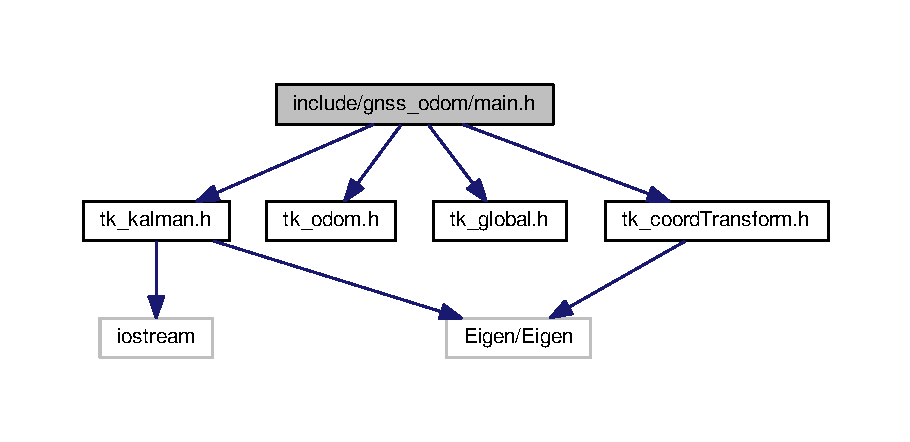
\includegraphics[width=350pt]{main_8h__incl}
\end{center}
\end{figure}
This graph shows which files directly or indirectly include this file\-:
\nopagebreak
\begin{figure}[H]
\begin{center}
\leavevmode
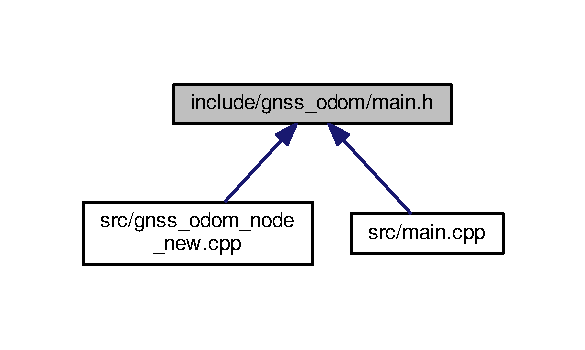
\includegraphics[width=281pt]{main_8h__dep__incl}
\end{center}
\end{figure}

\hypertarget{tk__coord_transform_8h}{\section{include/gnss\-\_\-odom/tk\-\_\-coord\-Transform.h File Reference}
\label{tk__coord_transform_8h}\index{include/gnss\-\_\-odom/tk\-\_\-coord\-Transform.\-h@{include/gnss\-\_\-odom/tk\-\_\-coord\-Transform.\-h}}
}
{\ttfamily \#include $<$Eigen/\-Eigen$>$}\\*
Include dependency graph for tk\-\_\-coord\-Transform.\-h\-:
\nopagebreak
\begin{figure}[H]
\begin{center}
\leavevmode
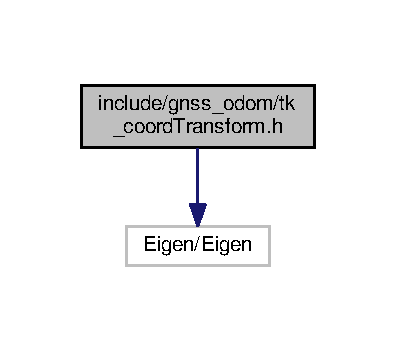
\includegraphics[width=190pt]{tk__coord_transform_8h__incl}
\end{center}
\end{figure}
This graph shows which files directly or indirectly include this file\-:
\nopagebreak
\begin{figure}[H]
\begin{center}
\leavevmode
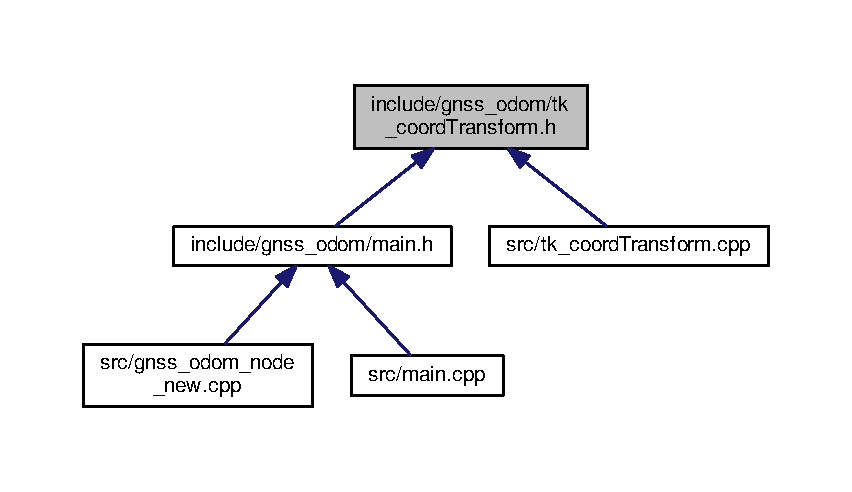
\includegraphics[width=350pt]{tk__coord_transform_8h__dep__incl}
\end{center}
\end{figure}
\subsection*{Classes}
\begin{DoxyCompactItemize}
\item 
struct \hyperlink{struct_coord_sys}{Coord\-Sys}
\item 
class \hyperlink{class_c_t_f}{C\-T\-F}
\end{DoxyCompactItemize}
\subsection*{Typedefs}
\begin{DoxyCompactItemize}
\item 
typedef struct \hyperlink{struct_coord_sys}{Coord\-Sys} \hyperlink{tk__coord_transform_8h_ad044a5a6d152b48925ad47ded0566b06}{C\-T}
\end{DoxyCompactItemize}


\subsection{Typedef Documentation}
\hypertarget{tk__coord_transform_8h_ad044a5a6d152b48925ad47ded0566b06}{\index{tk\-\_\-coord\-Transform.\-h@{tk\-\_\-coord\-Transform.\-h}!C\-T@{C\-T}}
\index{C\-T@{C\-T}!tk_coordTransform.h@{tk\-\_\-coord\-Transform.\-h}}
\subsubsection[{C\-T}]{\setlength{\rightskip}{0pt plus 5cm}typedef struct {\bf Coord\-Sys} {\bf C\-T}}}\label{tk__coord_transform_8h_ad044a5a6d152b48925ad47ded0566b06}

\hypertarget{tk__global_8h}{\section{include/gnss\-\_\-odom/tk\-\_\-global.h File Reference}
\label{tk__global_8h}\index{include/gnss\-\_\-odom/tk\-\_\-global.\-h@{include/gnss\-\_\-odom/tk\-\_\-global.\-h}}
}
This graph shows which files directly or indirectly include this file\-:
\nopagebreak
\begin{figure}[H]
\begin{center}
\leavevmode
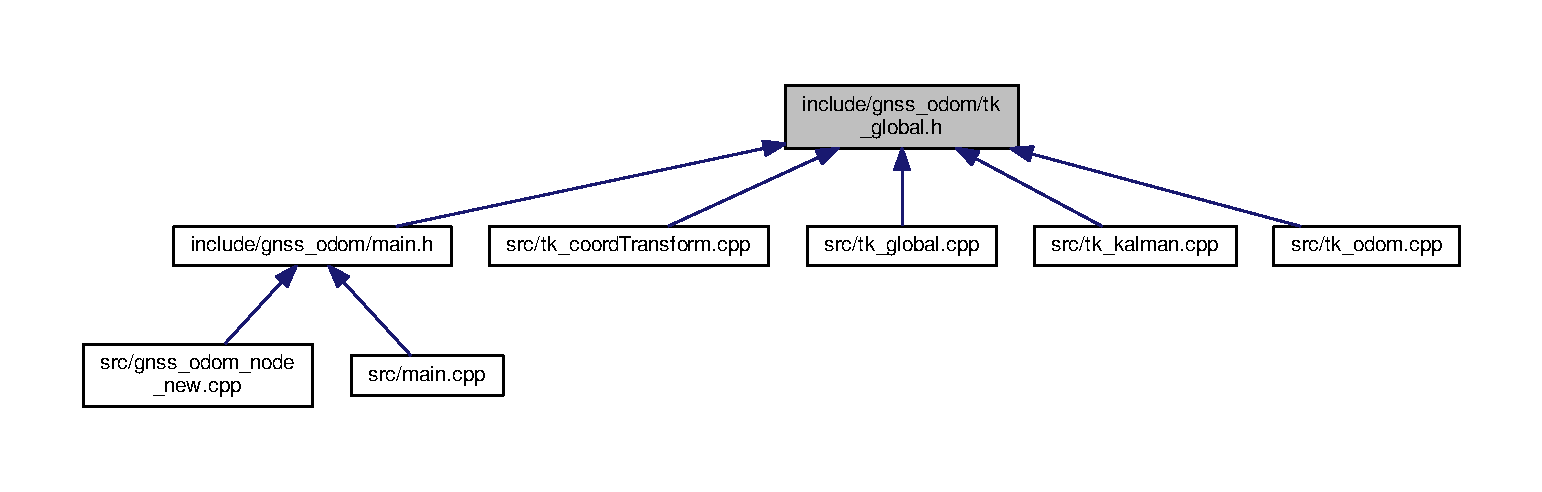
\includegraphics[width=350pt]{tk__global_8h__dep__incl}
\end{center}
\end{figure}
\subsection*{Variables}
\begin{DoxyCompactItemize}
\item 
const double \hyperlink{tk__global_8h_a0e9d57085f473ff892742782173b7a4d}{Len}
\item 
const double \hyperlink{tk__global_8h_a0a1d0930eaef243098b448c6ab044c8c}{k1}
\item 
const double \hyperlink{tk__global_8h_a462c2b139e125154ccdba2c9107e7e3e}{k2}
\item 
const double \hyperlink{tk__global_8h_a43016d873124d39034edb8cd164794db}{pi}
\item 
const double \hyperlink{tk__global_8h_ac058f9d1ca24439eb286a1f7005e5848}{lx}
\item 
const double \hyperlink{tk__global_8h_aaa1e0123e1baad493ec687904a428cbf}{ly}
\item 
const double \hyperlink{tk__global_8h_a32e31d87e8c8ecbeb7af7bc9332215fe}{lz}
\item 
const int \hyperlink{tk__global_8h_aaa0db75463dcb15429974ee99ced96ca}{x\-\_\-max}
\item 
const int \hyperlink{tk__global_8h_ab5631c1913883bb4c60d442f78c1f2ab}{y\-\_\-max}
\item 
const int \hyperlink{tk__global_8h_a38032630b7ea1b13e7b2539ab048d276}{x\-\_\-min}
\item 
const int \hyperlink{tk__global_8h_a886646055f10bf64b46ea25a0ea15935}{y\-\_\-min}
\item 
const double \hyperlink{tk__global_8h_a5d0b4770d96f3f117d176a0881b650f1}{min\-\_\-gpsx}
\item 
const double \hyperlink{tk__global_8h_a9a566fdf772ed1d10d4fd6208542027e}{min\-\_\-gpsy}
\item 
double \hyperlink{tk__global_8h_af26b544e9eeda32659fb48228ac6b97f}{theta} \mbox{[}132\mbox{]}\mbox{[}123\mbox{]}
\item 
double \hyperlink{tk__global_8h_a72f8637d05e25512d3961d3dd30f4559}{offset\-\_\-x} \mbox{[}132\mbox{]}\mbox{[}123\mbox{]}
\item 
double \hyperlink{tk__global_8h_ae82a027bc1485bcfb869eb436591c780}{offset\-\_\-y} \mbox{[}132\mbox{]}\mbox{[}123\mbox{]}
\item 
double \hyperlink{tk__global_8h_a4af6837c53e2ce993b55b4ada8fdf39d}{R\-T\-\_\-curr\-\_\-offset\-\_\-x}
\item 
double \hyperlink{tk__global_8h_ade9c28a8131302c3cc46eb3b5ebe4c3b}{R\-T\-\_\-curr\-\_\-offset\-\_\-y}
\item 
double \hyperlink{tk__global_8h_aa4272e9a9eb9a0ec62401dbc5f2c4d77}{R\-T\-\_\-curr\-\_\-theta}
\end{DoxyCompactItemize}


\subsection{Variable Documentation}
\hypertarget{tk__global_8h_a0a1d0930eaef243098b448c6ab044c8c}{\index{tk\-\_\-global.\-h@{tk\-\_\-global.\-h}!k1@{k1}}
\index{k1@{k1}!tk_global.h@{tk\-\_\-global.\-h}}
\subsubsection[{k1}]{\setlength{\rightskip}{0pt plus 5cm}const double k1}}\label{tk__global_8h_a0a1d0930eaef243098b448c6ab044c8c}
\hypertarget{tk__global_8h_a462c2b139e125154ccdba2c9107e7e3e}{\index{tk\-\_\-global.\-h@{tk\-\_\-global.\-h}!k2@{k2}}
\index{k2@{k2}!tk_global.h@{tk\-\_\-global.\-h}}
\subsubsection[{k2}]{\setlength{\rightskip}{0pt plus 5cm}const double k2}}\label{tk__global_8h_a462c2b139e125154ccdba2c9107e7e3e}
\hypertarget{tk__global_8h_a0e9d57085f473ff892742782173b7a4d}{\index{tk\-\_\-global.\-h@{tk\-\_\-global.\-h}!Len@{Len}}
\index{Len@{Len}!tk_global.h@{tk\-\_\-global.\-h}}
\subsubsection[{Len}]{\setlength{\rightskip}{0pt plus 5cm}const double Len}}\label{tk__global_8h_a0e9d57085f473ff892742782173b7a4d}
\hypertarget{tk__global_8h_ac058f9d1ca24439eb286a1f7005e5848}{\index{tk\-\_\-global.\-h@{tk\-\_\-global.\-h}!lx@{lx}}
\index{lx@{lx}!tk_global.h@{tk\-\_\-global.\-h}}
\subsubsection[{lx}]{\setlength{\rightskip}{0pt plus 5cm}const double lx}}\label{tk__global_8h_ac058f9d1ca24439eb286a1f7005e5848}
\hypertarget{tk__global_8h_aaa1e0123e1baad493ec687904a428cbf}{\index{tk\-\_\-global.\-h@{tk\-\_\-global.\-h}!ly@{ly}}
\index{ly@{ly}!tk_global.h@{tk\-\_\-global.\-h}}
\subsubsection[{ly}]{\setlength{\rightskip}{0pt plus 5cm}const double ly}}\label{tk__global_8h_aaa1e0123e1baad493ec687904a428cbf}
\hypertarget{tk__global_8h_a32e31d87e8c8ecbeb7af7bc9332215fe}{\index{tk\-\_\-global.\-h@{tk\-\_\-global.\-h}!lz@{lz}}
\index{lz@{lz}!tk_global.h@{tk\-\_\-global.\-h}}
\subsubsection[{lz}]{\setlength{\rightskip}{0pt plus 5cm}const double lz}}\label{tk__global_8h_a32e31d87e8c8ecbeb7af7bc9332215fe}
\hypertarget{tk__global_8h_a5d0b4770d96f3f117d176a0881b650f1}{\index{tk\-\_\-global.\-h@{tk\-\_\-global.\-h}!min\-\_\-gpsx@{min\-\_\-gpsx}}
\index{min\-\_\-gpsx@{min\-\_\-gpsx}!tk_global.h@{tk\-\_\-global.\-h}}
\subsubsection[{min\-\_\-gpsx}]{\setlength{\rightskip}{0pt plus 5cm}const double min\-\_\-gpsx}}\label{tk__global_8h_a5d0b4770d96f3f117d176a0881b650f1}
\hypertarget{tk__global_8h_a9a566fdf772ed1d10d4fd6208542027e}{\index{tk\-\_\-global.\-h@{tk\-\_\-global.\-h}!min\-\_\-gpsy@{min\-\_\-gpsy}}
\index{min\-\_\-gpsy@{min\-\_\-gpsy}!tk_global.h@{tk\-\_\-global.\-h}}
\subsubsection[{min\-\_\-gpsy}]{\setlength{\rightskip}{0pt plus 5cm}const double min\-\_\-gpsy}}\label{tk__global_8h_a9a566fdf772ed1d10d4fd6208542027e}
\hypertarget{tk__global_8h_a72f8637d05e25512d3961d3dd30f4559}{\index{tk\-\_\-global.\-h@{tk\-\_\-global.\-h}!offset\-\_\-x@{offset\-\_\-x}}
\index{offset\-\_\-x@{offset\-\_\-x}!tk_global.h@{tk\-\_\-global.\-h}}
\subsubsection[{offset\-\_\-x}]{\setlength{\rightskip}{0pt plus 5cm}double offset\-\_\-x\mbox{[}132\mbox{]}\mbox{[}123\mbox{]}}}\label{tk__global_8h_a72f8637d05e25512d3961d3dd30f4559}
\hypertarget{tk__global_8h_ae82a027bc1485bcfb869eb436591c780}{\index{tk\-\_\-global.\-h@{tk\-\_\-global.\-h}!offset\-\_\-y@{offset\-\_\-y}}
\index{offset\-\_\-y@{offset\-\_\-y}!tk_global.h@{tk\-\_\-global.\-h}}
\subsubsection[{offset\-\_\-y}]{\setlength{\rightskip}{0pt plus 5cm}double offset\-\_\-y\mbox{[}132\mbox{]}\mbox{[}123\mbox{]}}}\label{tk__global_8h_ae82a027bc1485bcfb869eb436591c780}
\hypertarget{tk__global_8h_a43016d873124d39034edb8cd164794db}{\index{tk\-\_\-global.\-h@{tk\-\_\-global.\-h}!pi@{pi}}
\index{pi@{pi}!tk_global.h@{tk\-\_\-global.\-h}}
\subsubsection[{pi}]{\setlength{\rightskip}{0pt plus 5cm}const double pi}}\label{tk__global_8h_a43016d873124d39034edb8cd164794db}
\hypertarget{tk__global_8h_a4af6837c53e2ce993b55b4ada8fdf39d}{\index{tk\-\_\-global.\-h@{tk\-\_\-global.\-h}!R\-T\-\_\-curr\-\_\-offset\-\_\-x@{R\-T\-\_\-curr\-\_\-offset\-\_\-x}}
\index{R\-T\-\_\-curr\-\_\-offset\-\_\-x@{R\-T\-\_\-curr\-\_\-offset\-\_\-x}!tk_global.h@{tk\-\_\-global.\-h}}
\subsubsection[{R\-T\-\_\-curr\-\_\-offset\-\_\-x}]{\setlength{\rightskip}{0pt plus 5cm}double R\-T\-\_\-curr\-\_\-offset\-\_\-x}}\label{tk__global_8h_a4af6837c53e2ce993b55b4ada8fdf39d}
\hypertarget{tk__global_8h_ade9c28a8131302c3cc46eb3b5ebe4c3b}{\index{tk\-\_\-global.\-h@{tk\-\_\-global.\-h}!R\-T\-\_\-curr\-\_\-offset\-\_\-y@{R\-T\-\_\-curr\-\_\-offset\-\_\-y}}
\index{R\-T\-\_\-curr\-\_\-offset\-\_\-y@{R\-T\-\_\-curr\-\_\-offset\-\_\-y}!tk_global.h@{tk\-\_\-global.\-h}}
\subsubsection[{R\-T\-\_\-curr\-\_\-offset\-\_\-y}]{\setlength{\rightskip}{0pt plus 5cm}double R\-T\-\_\-curr\-\_\-offset\-\_\-y}}\label{tk__global_8h_ade9c28a8131302c3cc46eb3b5ebe4c3b}
\hypertarget{tk__global_8h_aa4272e9a9eb9a0ec62401dbc5f2c4d77}{\index{tk\-\_\-global.\-h@{tk\-\_\-global.\-h}!R\-T\-\_\-curr\-\_\-theta@{R\-T\-\_\-curr\-\_\-theta}}
\index{R\-T\-\_\-curr\-\_\-theta@{R\-T\-\_\-curr\-\_\-theta}!tk_global.h@{tk\-\_\-global.\-h}}
\subsubsection[{R\-T\-\_\-curr\-\_\-theta}]{\setlength{\rightskip}{0pt plus 5cm}double R\-T\-\_\-curr\-\_\-theta}}\label{tk__global_8h_aa4272e9a9eb9a0ec62401dbc5f2c4d77}
\hypertarget{tk__global_8h_af26b544e9eeda32659fb48228ac6b97f}{\index{tk\-\_\-global.\-h@{tk\-\_\-global.\-h}!theta@{theta}}
\index{theta@{theta}!tk_global.h@{tk\-\_\-global.\-h}}
\subsubsection[{theta}]{\setlength{\rightskip}{0pt plus 5cm}double theta\mbox{[}132\mbox{]}\mbox{[}123\mbox{]}}}\label{tk__global_8h_af26b544e9eeda32659fb48228ac6b97f}
\hypertarget{tk__global_8h_aaa0db75463dcb15429974ee99ced96ca}{\index{tk\-\_\-global.\-h@{tk\-\_\-global.\-h}!x\-\_\-max@{x\-\_\-max}}
\index{x\-\_\-max@{x\-\_\-max}!tk_global.h@{tk\-\_\-global.\-h}}
\subsubsection[{x\-\_\-max}]{\setlength{\rightskip}{0pt plus 5cm}const int x\-\_\-max}}\label{tk__global_8h_aaa0db75463dcb15429974ee99ced96ca}
\hypertarget{tk__global_8h_a38032630b7ea1b13e7b2539ab048d276}{\index{tk\-\_\-global.\-h@{tk\-\_\-global.\-h}!x\-\_\-min@{x\-\_\-min}}
\index{x\-\_\-min@{x\-\_\-min}!tk_global.h@{tk\-\_\-global.\-h}}
\subsubsection[{x\-\_\-min}]{\setlength{\rightskip}{0pt plus 5cm}const int x\-\_\-min}}\label{tk__global_8h_a38032630b7ea1b13e7b2539ab048d276}
\hypertarget{tk__global_8h_ab5631c1913883bb4c60d442f78c1f2ab}{\index{tk\-\_\-global.\-h@{tk\-\_\-global.\-h}!y\-\_\-max@{y\-\_\-max}}
\index{y\-\_\-max@{y\-\_\-max}!tk_global.h@{tk\-\_\-global.\-h}}
\subsubsection[{y\-\_\-max}]{\setlength{\rightskip}{0pt plus 5cm}const int y\-\_\-max}}\label{tk__global_8h_ab5631c1913883bb4c60d442f78c1f2ab}
\hypertarget{tk__global_8h_a886646055f10bf64b46ea25a0ea15935}{\index{tk\-\_\-global.\-h@{tk\-\_\-global.\-h}!y\-\_\-min@{y\-\_\-min}}
\index{y\-\_\-min@{y\-\_\-min}!tk_global.h@{tk\-\_\-global.\-h}}
\subsubsection[{y\-\_\-min}]{\setlength{\rightskip}{0pt plus 5cm}const int y\-\_\-min}}\label{tk__global_8h_a886646055f10bf64b46ea25a0ea15935}

\hypertarget{tk__kalman_8h}{\section{include/gnss\-\_\-odom/tk\-\_\-kalman.h File Reference}
\label{tk__kalman_8h}\index{include/gnss\-\_\-odom/tk\-\_\-kalman.\-h@{include/gnss\-\_\-odom/tk\-\_\-kalman.\-h}}
}
{\ttfamily \#include $<$iostream$>$}\\*
{\ttfamily \#include $<$Eigen/\-Eigen$>$}\\*
Include dependency graph for tk\-\_\-kalman.\-h\-:
\nopagebreak
\begin{figure}[H]
\begin{center}
\leavevmode
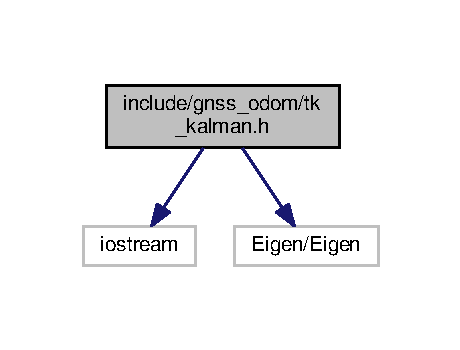
\includegraphics[width=221pt]{tk__kalman_8h__incl}
\end{center}
\end{figure}
This graph shows which files directly or indirectly include this file\-:
\nopagebreak
\begin{figure}[H]
\begin{center}
\leavevmode
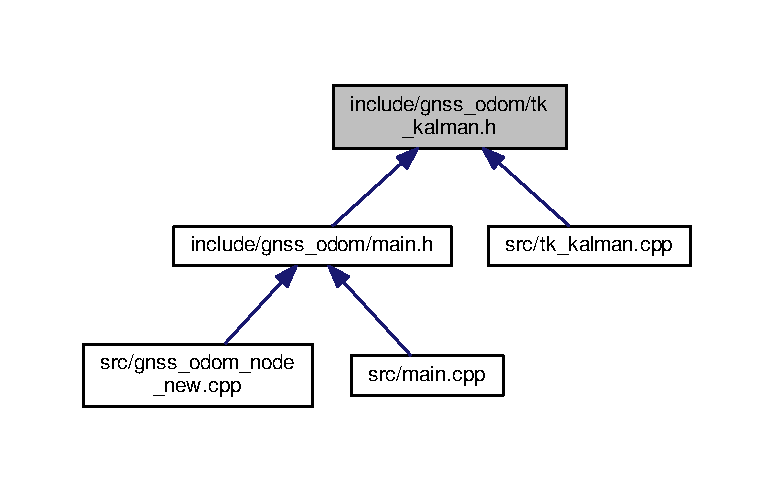
\includegraphics[width=350pt]{tk__kalman_8h__dep__incl}
\end{center}
\end{figure}
\subsection*{Classes}
\begin{DoxyCompactItemize}
\item 
struct \hyperlink{structkf___ft_qt}{kf\-\_\-\-Ft\-Qt}
\item 
struct \hyperlink{structkf___hk_rk}{kf\-\_\-\-Hk\-Rk}
\item 
struct \hyperlink{structkf___xk_pk}{kf\-\_\-\-Xk\-Pk}
\item 
class \hyperlink{class_k_f}{K\-F}
\end{DoxyCompactItemize}

\hypertarget{tk__odom_8h}{\section{include/gnss\-\_\-odom/tk\-\_\-odom.h File Reference}
\label{tk__odom_8h}\index{include/gnss\-\_\-odom/tk\-\_\-odom.\-h@{include/gnss\-\_\-odom/tk\-\_\-odom.\-h}}
}
This graph shows which files directly or indirectly include this file\-:
\nopagebreak
\begin{figure}[H]
\begin{center}
\leavevmode
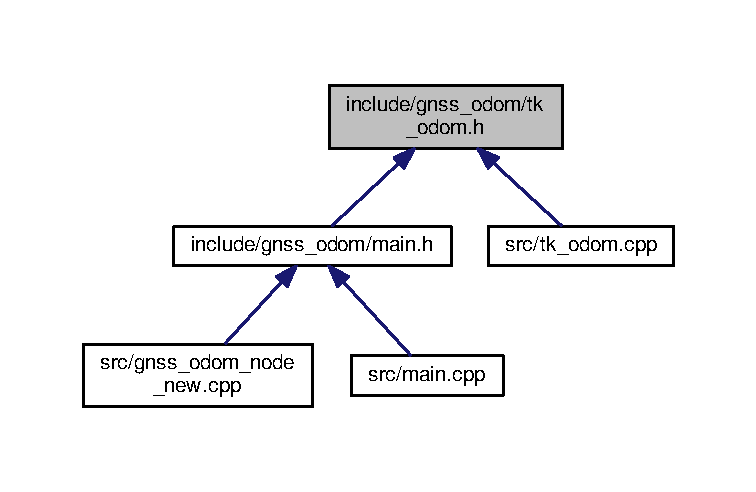
\includegraphics[width=350pt]{tk__odom_8h__dep__incl}
\end{center}
\end{figure}
\subsection*{Classes}
\begin{DoxyCompactItemize}
\item 
struct \hyperlink{structodom__res}{odom\-\_\-res}
\item 
class \hyperlink{class_o_d_o_m}{O\-D\-O\-M}
\end{DoxyCompactItemize}

\hypertarget{gnss__odom__node__new_8cpp}{\section{src/gnss\-\_\-odom\-\_\-node\-\_\-new.cpp File Reference}
\label{gnss__odom__node__new_8cpp}\index{src/gnss\-\_\-odom\-\_\-node\-\_\-new.\-cpp@{src/gnss\-\_\-odom\-\_\-node\-\_\-new.\-cpp}}
}
{\ttfamily \#include \char`\"{}ros/ros.\-h\char`\"{}}\\*
{\ttfamily \#include \char`\"{}af\-\_\-msgs/\-Fuse\-\_\-\-G\-\_\-\-O.\-h\char`\"{}}\\*
{\ttfamily \#include \char`\"{}af\-\_\-msgs/\-Gnss\-\_\-\-Odom\-\_\-lyz.\-h\char`\"{}}\\*
{\ttfamily \#include \char`\"{}Eigen/\-Eigen\char`\"{}}\\*
{\ttfamily \#include \char`\"{}main.\-h\char`\"{}}\\*
{\ttfamily \#include \char`\"{}iostream\char`\"{}}\\*
Include dependency graph for gnss\-\_\-odom\-\_\-node\-\_\-new.\-cpp\-:
\nopagebreak
\begin{figure}[H]
\begin{center}
\leavevmode
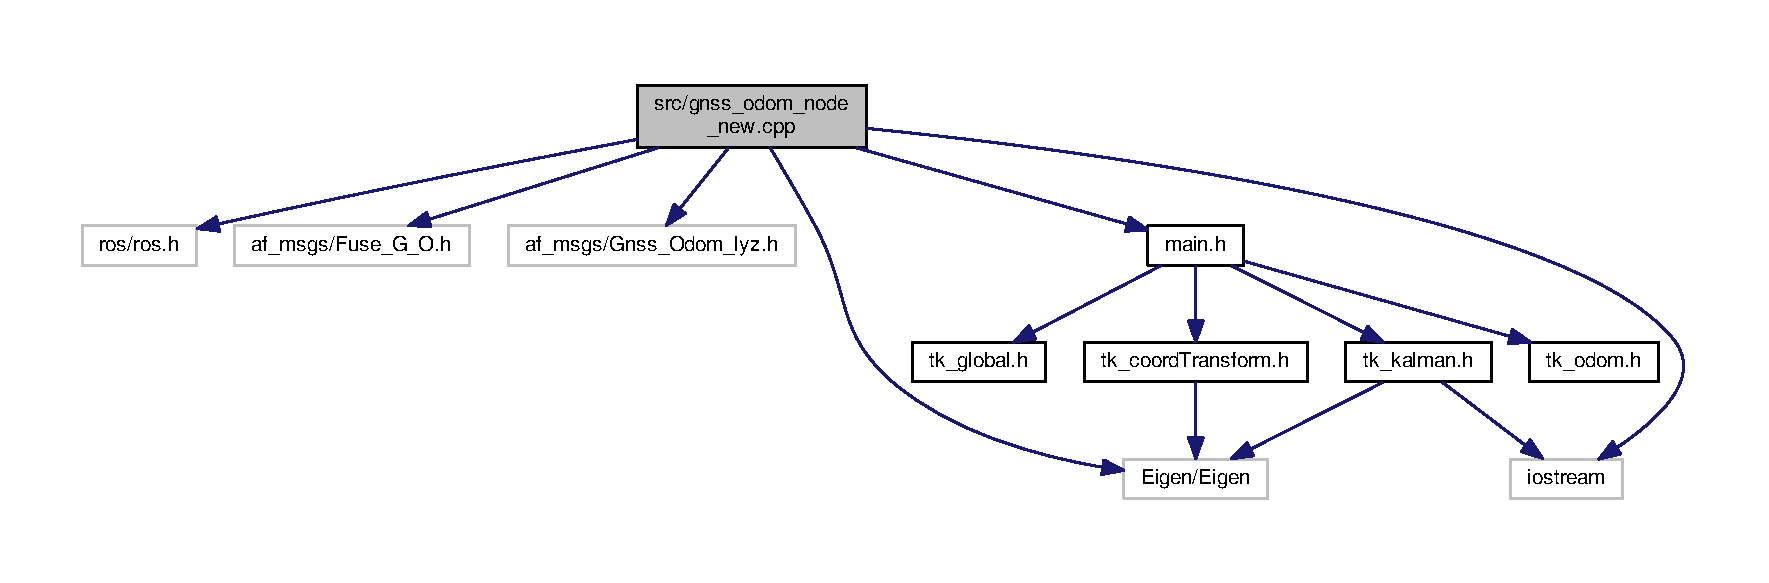
\includegraphics[width=350pt]{gnss__odom__node__new_8cpp__incl}
\end{center}
\end{figure}
\subsection*{Classes}
\begin{DoxyCompactItemize}
\item 
class \hyperlink{classfeedback}{feedback}
\end{DoxyCompactItemize}
\subsection*{Functions}
\begin{DoxyCompactItemize}
\item 
int \hyperlink{gnss__odom__node__new_8cpp_a3c04138a5bfe5d72780bb7e82a18e627}{main} (int argc, char $\ast$$\ast$argv)
\end{DoxyCompactItemize}
\subsection*{Variables}
\begin{DoxyCompactItemize}
\item 
af\-\_\-msgs\-::\-Gnss\-\_\-\-Odom\-\_\-lyz \hyperlink{gnss__odom__node__new_8cpp_a1a88dea45dbec17047b382f6522793e8}{output}
\item 
static int \hyperlink{gnss__odom__node__new_8cpp_a742204794ea328ba293fe59cec79b990}{m} = 2
\item 
\hyperlink{class_c_t_f}{C\-T\-F} \hyperlink{gnss__odom__node__new_8cpp_a111881b7f64a7c99315d76feb0e7ade5}{C\-T\-F\-\_\-}
\end{DoxyCompactItemize}


\subsection{Function Documentation}
\hypertarget{gnss__odom__node__new_8cpp_a3c04138a5bfe5d72780bb7e82a18e627}{\index{gnss\-\_\-odom\-\_\-node\-\_\-new.\-cpp@{gnss\-\_\-odom\-\_\-node\-\_\-new.\-cpp}!main@{main}}
\index{main@{main}!gnss_odom_node_new.cpp@{gnss\-\_\-odom\-\_\-node\-\_\-new.\-cpp}}
\subsubsection[{main}]{\setlength{\rightskip}{0pt plus 5cm}int main (
\begin{DoxyParamCaption}
\item[{int}]{argc, }
\item[{char $\ast$$\ast$}]{argv}
\end{DoxyParamCaption}
)}}\label{gnss__odom__node__new_8cpp_a3c04138a5bfe5d72780bb7e82a18e627}


\subsection{Variable Documentation}
\hypertarget{gnss__odom__node__new_8cpp_a111881b7f64a7c99315d76feb0e7ade5}{\index{gnss\-\_\-odom\-\_\-node\-\_\-new.\-cpp@{gnss\-\_\-odom\-\_\-node\-\_\-new.\-cpp}!C\-T\-F\-\_\-@{C\-T\-F\-\_\-}}
\index{C\-T\-F\-\_\-@{C\-T\-F\-\_\-}!gnss_odom_node_new.cpp@{gnss\-\_\-odom\-\_\-node\-\_\-new.\-cpp}}
\subsubsection[{C\-T\-F\-\_\-}]{\setlength{\rightskip}{0pt plus 5cm}{\bf C\-T\-F} C\-T\-F\-\_\-}}\label{gnss__odom__node__new_8cpp_a111881b7f64a7c99315d76feb0e7ade5}
\hypertarget{gnss__odom__node__new_8cpp_a742204794ea328ba293fe59cec79b990}{\index{gnss\-\_\-odom\-\_\-node\-\_\-new.\-cpp@{gnss\-\_\-odom\-\_\-node\-\_\-new.\-cpp}!m@{m}}
\index{m@{m}!gnss_odom_node_new.cpp@{gnss\-\_\-odom\-\_\-node\-\_\-new.\-cpp}}
\subsubsection[{m}]{\setlength{\rightskip}{0pt plus 5cm}int m = 2\hspace{0.3cm}{\ttfamily [static]}}}\label{gnss__odom__node__new_8cpp_a742204794ea328ba293fe59cec79b990}
\hypertarget{gnss__odom__node__new_8cpp_a1a88dea45dbec17047b382f6522793e8}{\index{gnss\-\_\-odom\-\_\-node\-\_\-new.\-cpp@{gnss\-\_\-odom\-\_\-node\-\_\-new.\-cpp}!output@{output}}
\index{output@{output}!gnss_odom_node_new.cpp@{gnss\-\_\-odom\-\_\-node\-\_\-new.\-cpp}}
\subsubsection[{output}]{\setlength{\rightskip}{0pt plus 5cm}af\-\_\-msgs\-::\-Gnss\-\_\-\-Odom\-\_\-lyz output}}\label{gnss__odom__node__new_8cpp_a1a88dea45dbec17047b382f6522793e8}

\hypertarget{main_8cpp}{\section{src/main.cpp File Reference}
\label{main_8cpp}\index{src/main.\-cpp@{src/main.\-cpp}}
}
{\ttfamily \#include $<$iostream$>$}\\*
{\ttfamily \#include \char`\"{}Eigen\char`\"{}}\\*
{\ttfamily \#include \char`\"{}stdlib.\-h\char`\"{}}\\*
{\ttfamily \#include \char`\"{}stdio.\-h\char`\"{}}\\*
{\ttfamily \#include \char`\"{}main.\-h\char`\"{}}\\*
Include dependency graph for main.\-cpp\-:
\nopagebreak
\begin{figure}[H]
\begin{center}
\leavevmode
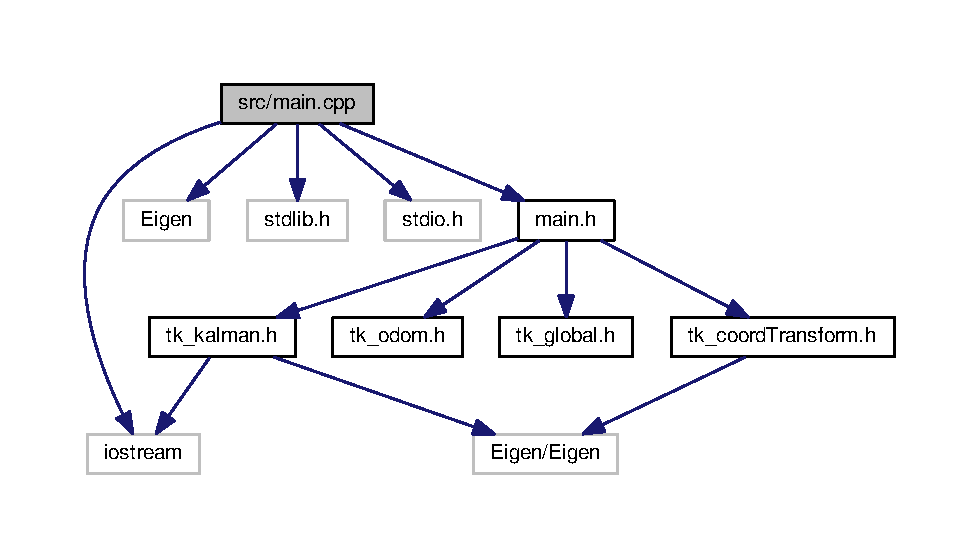
\includegraphics[width=350pt]{main_8cpp__incl}
\end{center}
\end{figure}
\subsection*{Functions}
\begin{DoxyCompactItemize}
\item 
int \hyperlink{main_8cpp_a840291bc02cba5474a4cb46a9b9566fe}{main} (void)
\end{DoxyCompactItemize}


\subsection{Function Documentation}
\hypertarget{main_8cpp_a840291bc02cba5474a4cb46a9b9566fe}{\index{main.\-cpp@{main.\-cpp}!main@{main}}
\index{main@{main}!main.cpp@{main.\-cpp}}
\subsubsection[{main}]{\setlength{\rightskip}{0pt plus 5cm}int main (
\begin{DoxyParamCaption}
\item[{void}]{}
\end{DoxyParamCaption}
)}}\label{main_8cpp_a840291bc02cba5474a4cb46a9b9566fe}

\hypertarget{tk__coord_transform_8cpp}{\section{src/tk\-\_\-coord\-Transform.cpp File Reference}
\label{tk__coord_transform_8cpp}\index{src/tk\-\_\-coord\-Transform.\-cpp@{src/tk\-\_\-coord\-Transform.\-cpp}}
}
{\ttfamily \#include \char`\"{}tk\-\_\-coord\-Transform.\-h\char`\"{}}\\*
{\ttfamily \#include \char`\"{}cmath\char`\"{}}\\*
{\ttfamily \#include \char`\"{}tk\-\_\-global.\-h\char`\"{}}\\*
{\ttfamily \#include $<$iostream$>$}\\*
Include dependency graph for tk\-\_\-coord\-Transform.\-cpp\-:
\nopagebreak
\begin{figure}[H]
\begin{center}
\leavevmode
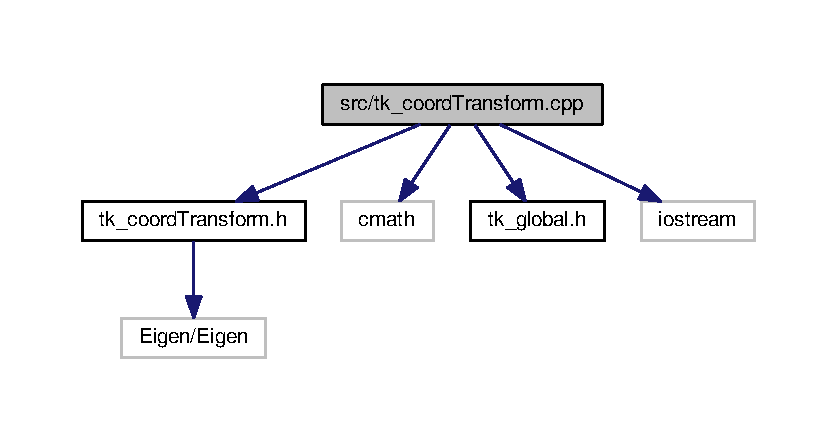
\includegraphics[width=350pt]{tk__coord_transform_8cpp__incl}
\end{center}
\end{figure}

\hypertarget{tk__global_8cpp}{\section{src/tk\-\_\-global.cpp File Reference}
\label{tk__global_8cpp}\index{src/tk\-\_\-global.\-cpp@{src/tk\-\_\-global.\-cpp}}
}
{\ttfamily \#include \char`\"{}tk\-\_\-global.\-h\char`\"{}}\\*
Include dependency graph for tk\-\_\-global.\-cpp\-:
\nopagebreak
\begin{figure}[H]
\begin{center}
\leavevmode
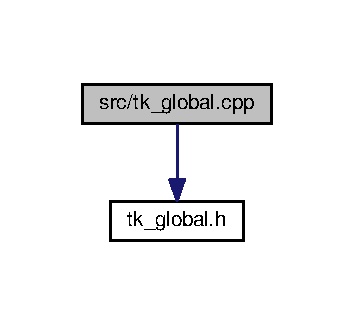
\includegraphics[width=170pt]{tk__global_8cpp__incl}
\end{center}
\end{figure}
\subsection*{Variables}
\begin{DoxyCompactItemize}
\item 
const double \hyperlink{tk__global_8cpp_a0e9d57085f473ff892742782173b7a4d}{Len} = 0.\-71
\item 
const double \hyperlink{tk__global_8cpp_a43016d873124d39034edb8cd164794db}{pi} = 3.\-141592653
\item 
const double \hyperlink{tk__global_8cpp_a0a1d0930eaef243098b448c6ab044c8c}{k1} = 0.\-42$\ast$\hyperlink{tk__global_8cpp_a43016d873124d39034edb8cd164794db}{pi}/4000.\-0/32.\-0
\item 
const double \hyperlink{tk__global_8cpp_a462c2b139e125154ccdba2c9107e7e3e}{k2} = 0.\-42$\ast$\hyperlink{tk__global_8cpp_a43016d873124d39034edb8cd164794db}{pi}/4000.\-0/32.\-0
\item 
const double \hyperlink{tk__global_8cpp_ac058f9d1ca24439eb286a1f7005e5848}{lx} = 0
\item 
const double \hyperlink{tk__global_8cpp_aaa1e0123e1baad493ec687904a428cbf}{ly} = 0
\item 
const double \hyperlink{tk__global_8cpp_a32e31d87e8c8ecbeb7af7bc9332215fe}{lz} = 0
\item 
const double \hyperlink{tk__global_8cpp_a5d0b4770d96f3f117d176a0881b650f1}{min\-\_\-gpsx} = 439742
\item 
const double \hyperlink{tk__global_8cpp_a9a566fdf772ed1d10d4fd6208542027e}{min\-\_\-gpsy} = 4425170
\item 
const int \hyperlink{tk__global_8cpp_aaa0db75463dcb15429974ee99ced96ca}{x\-\_\-max} = 131
\item 
const int \hyperlink{tk__global_8cpp_ab5631c1913883bb4c60d442f78c1f2ab}{y\-\_\-max} = 122
\item 
const int \hyperlink{tk__global_8cpp_a38032630b7ea1b13e7b2539ab048d276}{x\-\_\-min} = 0
\item 
const int \hyperlink{tk__global_8cpp_a886646055f10bf64b46ea25a0ea15935}{y\-\_\-min} = 0
\item 
double \hyperlink{tk__global_8cpp_a4af6837c53e2ce993b55b4ada8fdf39d}{R\-T\-\_\-curr\-\_\-offset\-\_\-x} = -\/74.\-046963263147532
\item 
double \hyperlink{tk__global_8cpp_ade9c28a8131302c3cc46eb3b5ebe4c3b}{R\-T\-\_\-curr\-\_\-offset\-\_\-y} = -\/4.\-953301447656681
\item 
double \hyperlink{tk__global_8cpp_aa4272e9a9eb9a0ec62401dbc5f2c4d77}{R\-T\-\_\-curr\-\_\-theta} = 0.\-055518275165770
\item 
double \hyperlink{tk__global_8cpp_a72f8637d05e25512d3961d3dd30f4559}{offset\-\_\-x} \mbox{[}132\mbox{]}\mbox{[}123\mbox{]}
\item 
double \hyperlink{tk__global_8cpp_ae82a027bc1485bcfb869eb436591c780}{offset\-\_\-y} \mbox{[}132\mbox{]}\mbox{[}123\mbox{]}
\item 
double \hyperlink{tk__global_8cpp_af26b544e9eeda32659fb48228ac6b97f}{theta} \mbox{[}132\mbox{]}\mbox{[}123\mbox{]}
\end{DoxyCompactItemize}


\subsection{Variable Documentation}
\hypertarget{tk__global_8cpp_a0a1d0930eaef243098b448c6ab044c8c}{\index{tk\-\_\-global.\-cpp@{tk\-\_\-global.\-cpp}!k1@{k1}}
\index{k1@{k1}!tk_global.cpp@{tk\-\_\-global.\-cpp}}
\subsubsection[{k1}]{\setlength{\rightskip}{0pt plus 5cm}const double k1 = 0.\-42$\ast${\bf pi}/4000.\-0/32.\-0}}\label{tk__global_8cpp_a0a1d0930eaef243098b448c6ab044c8c}
\hypertarget{tk__global_8cpp_a462c2b139e125154ccdba2c9107e7e3e}{\index{tk\-\_\-global.\-cpp@{tk\-\_\-global.\-cpp}!k2@{k2}}
\index{k2@{k2}!tk_global.cpp@{tk\-\_\-global.\-cpp}}
\subsubsection[{k2}]{\setlength{\rightskip}{0pt plus 5cm}const double k2 = 0.\-42$\ast${\bf pi}/4000.\-0/32.\-0}}\label{tk__global_8cpp_a462c2b139e125154ccdba2c9107e7e3e}
\hypertarget{tk__global_8cpp_a0e9d57085f473ff892742782173b7a4d}{\index{tk\-\_\-global.\-cpp@{tk\-\_\-global.\-cpp}!Len@{Len}}
\index{Len@{Len}!tk_global.cpp@{tk\-\_\-global.\-cpp}}
\subsubsection[{Len}]{\setlength{\rightskip}{0pt plus 5cm}const double Len = 0.\-71}}\label{tk__global_8cpp_a0e9d57085f473ff892742782173b7a4d}
\hypertarget{tk__global_8cpp_ac058f9d1ca24439eb286a1f7005e5848}{\index{tk\-\_\-global.\-cpp@{tk\-\_\-global.\-cpp}!lx@{lx}}
\index{lx@{lx}!tk_global.cpp@{tk\-\_\-global.\-cpp}}
\subsubsection[{lx}]{\setlength{\rightskip}{0pt plus 5cm}const double lx = 0}}\label{tk__global_8cpp_ac058f9d1ca24439eb286a1f7005e5848}
\hypertarget{tk__global_8cpp_aaa1e0123e1baad493ec687904a428cbf}{\index{tk\-\_\-global.\-cpp@{tk\-\_\-global.\-cpp}!ly@{ly}}
\index{ly@{ly}!tk_global.cpp@{tk\-\_\-global.\-cpp}}
\subsubsection[{ly}]{\setlength{\rightskip}{0pt plus 5cm}const double ly = 0}}\label{tk__global_8cpp_aaa1e0123e1baad493ec687904a428cbf}
\hypertarget{tk__global_8cpp_a32e31d87e8c8ecbeb7af7bc9332215fe}{\index{tk\-\_\-global.\-cpp@{tk\-\_\-global.\-cpp}!lz@{lz}}
\index{lz@{lz}!tk_global.cpp@{tk\-\_\-global.\-cpp}}
\subsubsection[{lz}]{\setlength{\rightskip}{0pt plus 5cm}const double lz = 0}}\label{tk__global_8cpp_a32e31d87e8c8ecbeb7af7bc9332215fe}
\hypertarget{tk__global_8cpp_a5d0b4770d96f3f117d176a0881b650f1}{\index{tk\-\_\-global.\-cpp@{tk\-\_\-global.\-cpp}!min\-\_\-gpsx@{min\-\_\-gpsx}}
\index{min\-\_\-gpsx@{min\-\_\-gpsx}!tk_global.cpp@{tk\-\_\-global.\-cpp}}
\subsubsection[{min\-\_\-gpsx}]{\setlength{\rightskip}{0pt plus 5cm}const double min\-\_\-gpsx = 439742}}\label{tk__global_8cpp_a5d0b4770d96f3f117d176a0881b650f1}
\hypertarget{tk__global_8cpp_a9a566fdf772ed1d10d4fd6208542027e}{\index{tk\-\_\-global.\-cpp@{tk\-\_\-global.\-cpp}!min\-\_\-gpsy@{min\-\_\-gpsy}}
\index{min\-\_\-gpsy@{min\-\_\-gpsy}!tk_global.cpp@{tk\-\_\-global.\-cpp}}
\subsubsection[{min\-\_\-gpsy}]{\setlength{\rightskip}{0pt plus 5cm}const double min\-\_\-gpsy = 4425170}}\label{tk__global_8cpp_a9a566fdf772ed1d10d4fd6208542027e}
\hypertarget{tk__global_8cpp_a72f8637d05e25512d3961d3dd30f4559}{\index{tk\-\_\-global.\-cpp@{tk\-\_\-global.\-cpp}!offset\-\_\-x@{offset\-\_\-x}}
\index{offset\-\_\-x@{offset\-\_\-x}!tk_global.cpp@{tk\-\_\-global.\-cpp}}
\subsubsection[{offset\-\_\-x}]{\setlength{\rightskip}{0pt plus 5cm}double offset\-\_\-x\mbox{[}132\mbox{]}\mbox{[}123\mbox{]}}}\label{tk__global_8cpp_a72f8637d05e25512d3961d3dd30f4559}
\hypertarget{tk__global_8cpp_ae82a027bc1485bcfb869eb436591c780}{\index{tk\-\_\-global.\-cpp@{tk\-\_\-global.\-cpp}!offset\-\_\-y@{offset\-\_\-y}}
\index{offset\-\_\-y@{offset\-\_\-y}!tk_global.cpp@{tk\-\_\-global.\-cpp}}
\subsubsection[{offset\-\_\-y}]{\setlength{\rightskip}{0pt plus 5cm}double offset\-\_\-y\mbox{[}132\mbox{]}\mbox{[}123\mbox{]}}}\label{tk__global_8cpp_ae82a027bc1485bcfb869eb436591c780}
\hypertarget{tk__global_8cpp_a43016d873124d39034edb8cd164794db}{\index{tk\-\_\-global.\-cpp@{tk\-\_\-global.\-cpp}!pi@{pi}}
\index{pi@{pi}!tk_global.cpp@{tk\-\_\-global.\-cpp}}
\subsubsection[{pi}]{\setlength{\rightskip}{0pt plus 5cm}const double pi = 3.\-141592653}}\label{tk__global_8cpp_a43016d873124d39034edb8cd164794db}
\hypertarget{tk__global_8cpp_a4af6837c53e2ce993b55b4ada8fdf39d}{\index{tk\-\_\-global.\-cpp@{tk\-\_\-global.\-cpp}!R\-T\-\_\-curr\-\_\-offset\-\_\-x@{R\-T\-\_\-curr\-\_\-offset\-\_\-x}}
\index{R\-T\-\_\-curr\-\_\-offset\-\_\-x@{R\-T\-\_\-curr\-\_\-offset\-\_\-x}!tk_global.cpp@{tk\-\_\-global.\-cpp}}
\subsubsection[{R\-T\-\_\-curr\-\_\-offset\-\_\-x}]{\setlength{\rightskip}{0pt plus 5cm}double R\-T\-\_\-curr\-\_\-offset\-\_\-x = -\/74.\-046963263147532}}\label{tk__global_8cpp_a4af6837c53e2ce993b55b4ada8fdf39d}
\hypertarget{tk__global_8cpp_ade9c28a8131302c3cc46eb3b5ebe4c3b}{\index{tk\-\_\-global.\-cpp@{tk\-\_\-global.\-cpp}!R\-T\-\_\-curr\-\_\-offset\-\_\-y@{R\-T\-\_\-curr\-\_\-offset\-\_\-y}}
\index{R\-T\-\_\-curr\-\_\-offset\-\_\-y@{R\-T\-\_\-curr\-\_\-offset\-\_\-y}!tk_global.cpp@{tk\-\_\-global.\-cpp}}
\subsubsection[{R\-T\-\_\-curr\-\_\-offset\-\_\-y}]{\setlength{\rightskip}{0pt plus 5cm}double R\-T\-\_\-curr\-\_\-offset\-\_\-y = -\/4.\-953301447656681}}\label{tk__global_8cpp_ade9c28a8131302c3cc46eb3b5ebe4c3b}
\hypertarget{tk__global_8cpp_aa4272e9a9eb9a0ec62401dbc5f2c4d77}{\index{tk\-\_\-global.\-cpp@{tk\-\_\-global.\-cpp}!R\-T\-\_\-curr\-\_\-theta@{R\-T\-\_\-curr\-\_\-theta}}
\index{R\-T\-\_\-curr\-\_\-theta@{R\-T\-\_\-curr\-\_\-theta}!tk_global.cpp@{tk\-\_\-global.\-cpp}}
\subsubsection[{R\-T\-\_\-curr\-\_\-theta}]{\setlength{\rightskip}{0pt plus 5cm}double R\-T\-\_\-curr\-\_\-theta = 0.\-055518275165770}}\label{tk__global_8cpp_aa4272e9a9eb9a0ec62401dbc5f2c4d77}
\hypertarget{tk__global_8cpp_af26b544e9eeda32659fb48228ac6b97f}{\index{tk\-\_\-global.\-cpp@{tk\-\_\-global.\-cpp}!theta@{theta}}
\index{theta@{theta}!tk_global.cpp@{tk\-\_\-global.\-cpp}}
\subsubsection[{theta}]{\setlength{\rightskip}{0pt plus 5cm}double theta\mbox{[}132\mbox{]}\mbox{[}123\mbox{]}}}\label{tk__global_8cpp_af26b544e9eeda32659fb48228ac6b97f}
\hypertarget{tk__global_8cpp_aaa0db75463dcb15429974ee99ced96ca}{\index{tk\-\_\-global.\-cpp@{tk\-\_\-global.\-cpp}!x\-\_\-max@{x\-\_\-max}}
\index{x\-\_\-max@{x\-\_\-max}!tk_global.cpp@{tk\-\_\-global.\-cpp}}
\subsubsection[{x\-\_\-max}]{\setlength{\rightskip}{0pt plus 5cm}const int x\-\_\-max = 131}}\label{tk__global_8cpp_aaa0db75463dcb15429974ee99ced96ca}
\hypertarget{tk__global_8cpp_a38032630b7ea1b13e7b2539ab048d276}{\index{tk\-\_\-global.\-cpp@{tk\-\_\-global.\-cpp}!x\-\_\-min@{x\-\_\-min}}
\index{x\-\_\-min@{x\-\_\-min}!tk_global.cpp@{tk\-\_\-global.\-cpp}}
\subsubsection[{x\-\_\-min}]{\setlength{\rightskip}{0pt plus 5cm}const int x\-\_\-min = 0}}\label{tk__global_8cpp_a38032630b7ea1b13e7b2539ab048d276}
\hypertarget{tk__global_8cpp_ab5631c1913883bb4c60d442f78c1f2ab}{\index{tk\-\_\-global.\-cpp@{tk\-\_\-global.\-cpp}!y\-\_\-max@{y\-\_\-max}}
\index{y\-\_\-max@{y\-\_\-max}!tk_global.cpp@{tk\-\_\-global.\-cpp}}
\subsubsection[{y\-\_\-max}]{\setlength{\rightskip}{0pt plus 5cm}const int y\-\_\-max = 122}}\label{tk__global_8cpp_ab5631c1913883bb4c60d442f78c1f2ab}
\hypertarget{tk__global_8cpp_a886646055f10bf64b46ea25a0ea15935}{\index{tk\-\_\-global.\-cpp@{tk\-\_\-global.\-cpp}!y\-\_\-min@{y\-\_\-min}}
\index{y\-\_\-min@{y\-\_\-min}!tk_global.cpp@{tk\-\_\-global.\-cpp}}
\subsubsection[{y\-\_\-min}]{\setlength{\rightskip}{0pt plus 5cm}const int y\-\_\-min = 0}}\label{tk__global_8cpp_a886646055f10bf64b46ea25a0ea15935}

\hypertarget{tk__kalman_8cpp}{\section{src/tk\-\_\-kalman.cpp File Reference}
\label{tk__kalman_8cpp}\index{src/tk\-\_\-kalman.\-cpp@{src/tk\-\_\-kalman.\-cpp}}
}
{\ttfamily \#include \char`\"{}tk\-\_\-kalman.\-h\char`\"{}}\\*
{\ttfamily \#include \char`\"{}tk\-\_\-global.\-h\char`\"{}}\\*
Include dependency graph for tk\-\_\-kalman.\-cpp\-:
\nopagebreak
\begin{figure}[H]
\begin{center}
\leavevmode
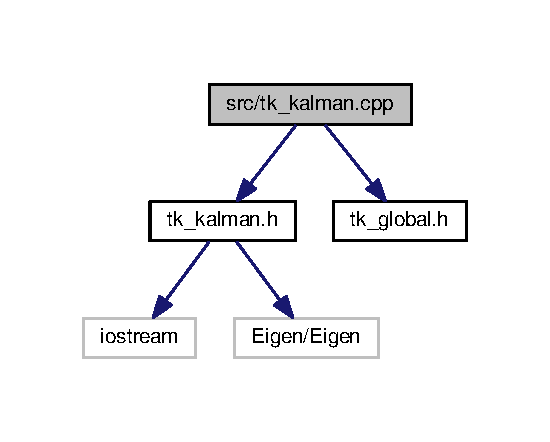
\includegraphics[width=264pt]{tk__kalman_8cpp__incl}
\end{center}
\end{figure}

\hypertarget{tk__odom_8cpp}{\section{src/tk\-\_\-odom.cpp File Reference}
\label{tk__odom_8cpp}\index{src/tk\-\_\-odom.\-cpp@{src/tk\-\_\-odom.\-cpp}}
}
{\ttfamily \#include \char`\"{}tk\-\_\-odom.\-h\char`\"{}}\\*
{\ttfamily \#include \char`\"{}tk\-\_\-global.\-h\char`\"{}}\\*
{\ttfamily \#include \char`\"{}math.\-h\char`\"{}}\\*
{\ttfamily \#include \char`\"{}iostream\char`\"{}}\\*
Include dependency graph for tk\-\_\-odom.\-cpp\-:
\nopagebreak
\begin{figure}[H]
\begin{center}
\leavevmode
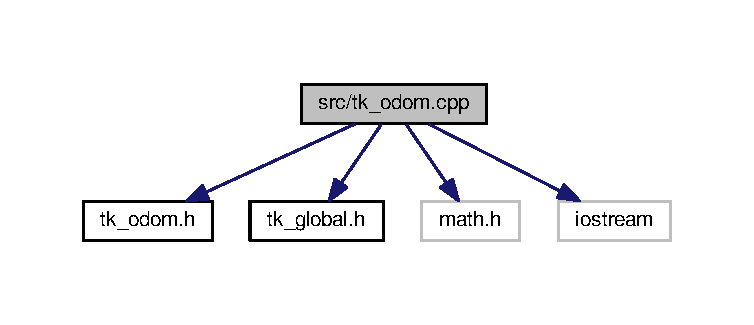
\includegraphics[width=350pt]{tk__odom_8cpp__incl}
\end{center}
\end{figure}

%--- End generated contents ---

% Index
\newpage
\phantomsection
\addcontentsline{toc}{chapter}{Index}
\printindex

\end{document}
